\section{FedECS-LT, component by component}\label{ch:method}

FedECS-LT (Exact Class Statistics for Long-Tailed federated learning) keeps GeFL-F's three stages and its frozen
extractor. It obtains the class-specific quantities of the generator and the last layer from statistics that secure
aggregation computes exactly (\cref{ch:sums}), the \emph{exact class statistics}, instead of from parameters
estimated by FedAvg. It also changes how the heads are trained, and it adds a last step that sets every last layer.
\Cref{fig:s-overview} is the paper's overview; this chapter takes the components in pipeline order.

\begin{figure}[t]
\centering
\includegraphics[width=\linewidth]{\genpath/figures/fig_overview.pdf}
\caption{The paper's overview of FedECS-LT. C: computed by each client; S: computed by the server; SA: summed over
the clients by secure aggregation. Read it left to right: statistics after Stage I, the generator chosen by the gate
(Stage II), the moment correction, the heads (Stage III), and the exact readout last.}
\label{fig:s-overview}
\end{figure}

\subsection{Statistics release}\label{sec:s-stats}

\paragraph{What it answers} Every later component needs the class means and spreads of the features. They are
functions of sums, so they can be computed exactly (\cref{ch:sums}).

\paragraph{How it works} After Stage I, client $k$ computes for every class $c$ its count $n_{kc}$, its feature sum
$S^{(1)}_{kc}$ and its sum of squared feature norms $S^{(2)}_{kc}$. Secure aggregation returns the totals, and the
server forms (\texttt{fedecs.moments\_from\_sums})
\[
\mu_c=S^{(1)}_c/n_c,\qquad V_c=S^{(2)}_c/n_c-\|\mu_c\|^2 .
\]
$\mu_c$ is the mean feature of class $c$, a vector of $d=2560$ numbers, and $V_c$ its \emph{spread}, the mean squared
distance of a class-$c$ feature from $\mu_c$. In this text ``spread'' without a qualifier always means $V_c$, a squared
quantity; the \emph{logit spread} of \cref{sec:s-spread} is a different measurement.

\paragraph{Cost} Each client sends $C(d+2)$ numbers once: for each class, one count, one number for the sum of squared
norms, and $d$ for the feature sum. On CIFAR-10 that is $10\cdot2562=25{,}620$ numbers.

\subsection{The generator}\label{sec:s-gen}

\paragraph{The mean-anchored generator} This is the default branch. It generates a class-$y$ feature as
\[
\tilde h=\mathrm{ReLU}\big(\mu_y+\mathrm{dec}(z,\,A\mu_y)\big),\qquad z\sim\mathcal N(0,I),
\]
where $\mathrm{dec}$ is the decoder network and $A$ a projection shared by all classes. The exact mean $\mu_y$ is
added directly, and the decoder only has to model the deviation from it. The class enters only through the vector
$\mu_y$, which the server computed exactly, and through $A$, which every class shares. The generator therefore has no
class row and no other class-specific parameter: the contraction of \cref{sec:s-decay} has nothing to shrink. It is
trained by FedAvg with Adam, like GeFL-F's.

\paragraph{What an anchor can express} An anchored generator can make two classes only as different as their means
allow. The paper's appendix bounds the difference by the \emph{Wasserstein distance} $W_1$ between the two generated
distributions, the least average distance by which the points of one must be moved to turn it into the other:
\[
W_1(G_c,G_{c'})\le(1+L\|A\|_2)\,\|\mu_c-\mu_{c'}\|,
\]
where $L$ is the Lipschitz constant of the decoder in its second input (how much its output can change per unit change
of $A\mu$) and $\|A\|_2$ the largest stretch of the projection. The proof idea: generate both classes from the same
noise $z$; then each generated pair differs by at most $\|\mu_c-\mu_{c'}\|$ from the anchor plus $L\|A\|_2$ times that
from the decoder, and the ReLU never increases a distance. In words: when two class means are close, the anchored
generator cannot make the classes far apart unless $L\|A\|_2$ is large, and nothing in training controls that factor.
GeFL-F's class rows have no such limit, because a class row can encode a difference between classes that the mean does
not show.

\paragraph{The separation gate} So the server first measures how separated the means are, relative to the spread
(\texttt{fedecs.separation\_F}):
\[
F=\frac{\frac1C\sum_c\|\mu_c-\bar\mu\|^2}{\frac1C\sum_c V_c},\qquad \bar\mu=\frac1C\sum_c\mu_c .
\]
The numerator is the spread of the class means around their centre, the denominator the average spread within a
class. (It is a form of the ratio that linear discriminant analysis maximises, which \cref{sec:s-readout} explains.)
If $F\ge F_0=0.05$, the server uses the mean-anchored generator; otherwise it falls back to GeFL-F's generator, with
class rows averaged by CCWA. The threshold was fixed during the method's development and not swept.

A toy case: two classes on a line with means $-1$ and $+1$, each with spread $V=4$ (standard deviation 2). Then
$\bar\mu=0$, the numerator is $(1+1)/2=1$, the denominator $4$, and $F=0.25$. Over pairs of distinct classes, two
class means are on average $\sqrt{2FC/(C-1)}$ root-mean-square spreads apart (an appendix identity): here
$\sqrt{2\cdot0.25\cdot2}=1$, and indeed the means are 2 apart and the spread's root is 2. The threshold $F_0=0.05$ with
ten classes means $\sqrt{2\cdot0.05\cdot10/9}\approx0.33$: class means a third of a spread apart. The running example
has $F\approx0.080$ (seed 3, run log), so two CIFAR-10 class means are on average about 0.42 spreads apart: in the
frozen feature space the classes overlap heavily, and yet the anchor branch is chosen. Across all the paper's runs $F$
ranges from \R{gate/F/min_all} to \R{gate/F/max_all}, and the gate chose class rows on \R{gate/rows_all} (the
shared-model protocol is described in \cref{ch:design}).

\paragraph{The fallback: class rows with CCWA} When the gate finds the means too close, the generator keeps GeFL-F's
class rows, but the server averages each row only over the clients that hold the class, weighted by how much of it
they hold:
\[
r_c\leftarrow\frac{\sum_k E(n_{kc})\,r_{k,c}}{\sum_k E(n_{kc})},\qquad E(n)=\frac{1-\beta^n}{1-\beta},\quad\beta=0.999 .
\]
$E(n)$ is the \emph{effective number of samples} (a function of a count, not the expectation $\E$), and this $\beta$
is CCWA's own constant, unrelated to Adam's $\beta_2$ although equal in value. $E(n)$ is zero for a client without the
class, so non-holders drop out and the term $\bar g^{-}_c$ of the contraction lemma disappears. It is close to $n$ for small
$n$ and saturates at $1/(1-\beta)=1000$, so one large client cannot dominate a class. For class 9 of the running
example, client 7 (63 images) gets weight $E(63)\approx61.1$, client 1 (4 images) gets $E(4)\approx4.0$, and clients 2
and 5 get zero. For class 1, client 7's 2,803 images give $E(2803)\approx940$, not 2,803. Both sums are computed by
secure aggregation, so the server never sees a single client's counts.

\subsection{Moment correction}\label{sec:s-mc}

\paragraph{What it answers} Even a generator anchored to the right mean can produce features with the wrong spread,
too concentrated or too dispersed, and a class-rows generator can drift in mean too. The server knows the exact mean
$\mu_c$ and spread $V_c$, so it can correct the generated features to match them.

\paragraph{How it works} After Stage II the server draws 500 features per class from the generator, measures their
mean $\tilde\mu_c$ and spread $\tilde V_c$, and from then on corrects every generated feature of class $c$ by
(\texttt{fedecs.MomentCalibratedGen})
\[
\tilde h\leftarrow\mathrm{ReLU}\big(\mu_c+s_c(\tilde h-\tilde\mu_c)\big),\qquad
s_c=\mathrm{clip}\Big(\sqrt{V_c/\tilde V_c},\;0.1,\;10\Big).
\]
The map first moves the generated class to its exact mean, then rescales the deviations so that their spread becomes
the exact one. One scale $s_c$ multiplies every coordinate, so the correction matches the total spread, not the shape
of the class: a class that is too wide in one direction and too narrow in another keeps that imbalance.

\paragraph{A worked example} Take one coordinate, for illustration, with exact mean $0.5$ and exact spread $0.25$,
and generated features of mean $0.8$ and spread $0.0625$. Then $s_c=\sqrt{0.25/0.0625}=2$. A generated value $0.7$
becomes $0.5+2(0.7-0.8)=0.3$; a generated value $0.5$ becomes $0.5+2(0.5-0.8)=-0.1$, which the ReLU sets to $0$. Before
the ReLU the corrected values have exactly the target mean and spread. The ReLU raises the negative ones to zero, which
pulls them toward the mean, so the corrected spread comes out a little below the target.

\paragraph{Why this map} Without the final ReLU and the clipping, this is the map that reaches the exact mean and
spread while moving the generated features as little as possible (an appendix lemma). The proof idea: for a map $M$
with the required mean and spread, the expected squared displacement $\E\|M(X)-X\|^2$ is fixed except for one term,
$-2\E\langle M(X)-\mu_c,\,X-\tilde\mu_c\rangle$, and the Cauchy--Schwarz inequality says this term is smallest when
$M(X)-\mu_c$ is a positive multiple of $X-\tilde\mu_c$, which is the map above. The ReLU keeps features non-negative, as
real features after a ReLU are, and the clipping prevents extreme rescaling, so in practice the moments match only
approximately. Across every class and run of the long-tailed benchmarks, the corrected spread is \R{main/mc_spread_lo}
to \R{main/mc_spread_hi} times the exact spread $V_c$ (median \R{main/mc_spread_med}), below one as the example
predicts.

\paragraph{Cost} The server sends $(\mu_c,\tilde\mu_c,s_c)$ to the clients once; each client holds the generator and
corrects its own samples.

\paragraph{What the evidence says} Matching moments is not the same as making features recognisable. The fidelity
table (\cref{tab:s-fidelity}) shows that on CIFAR-10-LT the correction raises the referee's accuracy on the head
classes from \R{main/cifar10/FedECS-LT/fidelity_head} to \R{main/cifar10/FedECS-LT/fidelity_mc_head}, and changes the
tail classes' from \R{main/cifar10/FedECS-LT/fidelity_tail} to \R{main/cifar10/FedECS-LT/fidelity_mc_tail} and the
mean from \R{main/cifar10/FedECS-LT/fidelity_all} to \R{main/cifar10/FedECS-LT/fidelity_mc_all}. The tail and mean
changes are within one standard deviation over the seeds. On CIFAR-100-LT the mean is unchanged
(\R{main/cifar100/FedECS-LT/fidelity_all} and \R{main/cifar100/FedECS-LT/fidelity_mc_all}). The component ablation
(\cref{sec:s-ablations}) finds no benefit for accuracy: the full method minus its variant without the correction is
\R{comp/cifar10/w/o moment correction/er_drop} points with the readout on CIFAR-10-LT.

\subsection{The heads}\label{sec:s-heads}

Each Stage-III round, client $k$, holding $n_k$ real images, first takes $T_s\lfloor n_k/B\rfloor$ SGD steps on batches
of $B$ corrected generated features ($B=128$ on CIFAR), that is, $T_s$ epochs of the size of its real data, and then
trains $T_r=5$ epochs on its real features. Each phase starts a fresh SGD optimiser (learning rate 0.1, no momentum).
Three things differ from GeFL-F.

\paragraph{Logit adjustment in the real phase} The real phase uses $\ell(f+\tau\log\hat\pi_k,y)$ with $\tau=1$ and the
client's add-one smoothed class frequencies $\hat\pi_k$. On a head trained only on real data this would add no
information about absent classes (\cref{sec:s-lastlayer}), but here it is applied in the real phase only, between
synthetic phases without it, so the reparametrisation lemma does not cover it. The paper gives two reasons for it:
without it, cross-entropy keeps pushing the absent classes' logits down during the real phase (\cref{sec:s-spread}),
and it can change what the body learns. $\hat\pi_k$ is the client's own frequencies, not an exact class statistic. How
much logit adjustment contributes is not resolved: its ablation finished one seed per benchmark
(\cref{sec:s-ablations}).

\paragraph{Consensus soft labels in the synthetic phase} The synthetic phase still draws labels uniformly, but the
target is no longer the one-hot label alone. For a generated feature $\tilde h$ with label $y$,
\[
t(\tilde h)=(1-\omega)\,\mathbf 1_y+\omega\,\frac1{10}\sum_{g=1}^{10}\mathrm{softmax}\big(f_g(\tilde h)\big),\qquad\omega=0.5,
\]
where $\mathbf 1_y$ is the one-hot vector of $y$ and $f_g$ the current head of architecture $g$. The second term is the
federation's averaged prediction on that feature, the same kind of target as FedDF's distillation. If a generated
``class 9'' feature looks to the federation's heads like class 3 with probability 0.4 and like class 9 with 0.05, its
target puts $0.5+0.5\cdot0.05=0.525$ on class 9 and $0.2$ on class 3. The weight $\omega=0.5$ was fixed in development.

This answers the third loss of \cref{ch:diagnosis}: the target now depends on the feature, so the premise of the
label-free lemma, a label independent of the feature, no longer holds, and the synthetic phase need not pull the logits
together. The intent is that the target follows what the feature carries instead of forcing a label it may not
support, and that every head learns from the ensemble of all ten architectures; the ablation confirms that consensus soft labels
improve accuracy: removing them costs \R{comp/cifar10/w/o consensus soft labels/er_drop} points with the readout on
CIFAR-10-LT and \R{comp/cifar100/w/o consensus soft labels/er_drop} on CIFAR-100-LT, the one component effect the
ablation resolves (\cref{sec:s-ablations}).

\paragraph{How the consensus is computed} The average is computed by one secure sum per round. Every client
regenerates the same pool of generated features from a seed the server sends. Writing $\mathrm{arch}(k)$ for the architecture
of client $k$, it returns $w_k\,\mathrm{softmax}(f_{\mathrm{arch}(k)}(\tilde h))$ for every feature of the pool, with
$w_k=1/(10\cdot|\{j:\mathrm{arch}(j)=\mathrm{arch}(k)\}|)$, one over ten times the number of clients of its own architecture. The secure sum of
these is the average above. The pool is as large as the largest client's synthetic phase, $T_s\lfloor n_k/B\rfloor B$
(\texttt{fedecs.csl\_pool\_size}): in the running example, client 7 with 4,538 images gives
$10\cdot35\cdot128=44{,}800$ features, so every client returns $448{,}000$ numbers per round. For this every client also
receives every architecture's current head each round, which FedAvg within an architecture would not require.

\paragraph{Ten synthetic epochs} $T_s=10$ instead of GeFL-F's 1. This is more computation, not a statistic, and the
paper lists it as one of the method's changes.

\subsection{The exact readout}\label{sec:s-readout}

This component gets the most space, because \cref{ch:results} shows that it carries most of the gain.

\paragraph{What it answers} \Cref{sec:s-lastlayer} showed that a last layer trained on one client knows nothing about
the classes the client lacks, and that a last layer computed from sums over all clients equals the one computed on
pooled data. The exact readout is such a last layer: after Stage III, every architecture's trained last layer is
replaced by a classifier computed from aggregated statistics of the embeddings.

\paragraph{The classifier} Suppose the embeddings $e$ of each class $c$ are Gaussian with mean $\nu_c$ and a covariance
$\Sigma$ shared by all classes, and every class is equally likely. Then the most probable class for an embedding $e$
maximises the log-density of $e$ under class $c$,
\[
\log \mathcal N(e;\nu_c,\Sigma)=-\tfrac12(e-\nu_c)^\top\Sigma^{-1}(e-\nu_c)+\text{const}
= e^\top\Sigma^{-1}\nu_c-\tfrac12\nu_c^\top\Sigma^{-1}\nu_c-\tfrac12e^\top\Sigma^{-1}e+\text{const}.
\]
The term $-\frac12e^\top\Sigma^{-1}e$ is the same for every class, so it does not affect which class wins. What is left
is linear in $e$: the logit of class $c$ is $w_c^\top e+b_c$ with
\[
w_c=\Sigma^{-1}\nu_c,\qquad b_c=-\tfrac12\,\nu_c^\top\Sigma^{-1}\nu_c .
\]
This is linear discriminant analysis (LDA). The usual LDA adds $\log\pi_c$, the class prior, to $b_c$, which favours
frequent classes. Leaving it out makes the classifier \emph{class-balanced}: it treats every class as equally likely,
which is what balanced accuracy rewards. The classifier is the nearest class mean in the Mahalanobis distance
$(e-\nu_c)^\top\Sigma^{-1}(e-\nu_c)$, a distance that measures each direction in units of the spread along it. LDA's
directions are also those that maximise the ratio of the spread between class means to the spread within classes,
which is why the gate's $F$ was called a form of its ratio.

\paragraph{A two-dimensional example} Take two classes with means $\nu_A=(1,1)$ and $\nu_B=(0,0)$ and the shared
covariance $\Sigma=\mathrm{diag}(1,\,0.25)$: the second coordinate is four times less noisy than the first. Then
$\Sigma^{-1}=\mathrm{diag}(1,4)$, $w_A=(1,4)$, $b_A=-\frac12(1+4)=-2.5$, $w_B=0$, $b_B=0$, and class A wins when
$x+4y>2.5$. The nearest-mean rule would instead decide by $x+y>1$. For the point $e=(1.2,\,0.3)$ the nearest-mean rule
says A, since $1.5>1$, but LDA says B, since $1.2+1.2=2.4<2.5$. The point is far from A along the precise coordinate
and close to B there, and LDA trusts that coordinate more (\cref{fig:s-lda}).

\begin{figure}[t]
\centering
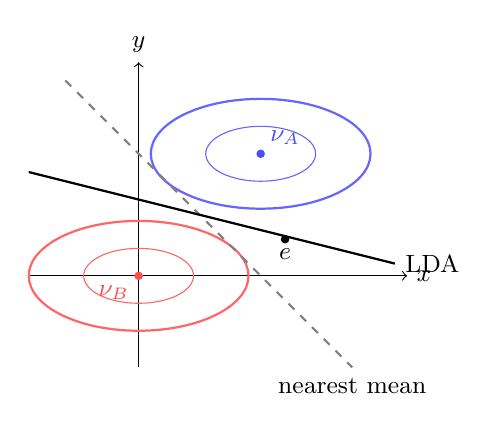
\begin{tikzpicture}[scale=1.55,font=\small]
\draw[->] (-0.9,0) -- (2.2,0) node[right]{$x$};
\draw[->] (0,-0.75) -- (0,1.75) node[above]{$y$};
\foreach \cx/\cy/\col in {1/1/blue!60,0/0/red!60}{
  \draw[\col,thick] (\cx,\cy) ellipse (0.9 and 0.45);
  \draw[\col] (\cx,\cy) ellipse (0.45 and 0.225);}
\fill[blue!70] (1,1) circle (0.035) node[above right]{$\nu_A$};
\fill[red!70] (0,0) circle (0.035) node[below left]{$\nu_B$};
\draw[gray,dashed,thick] (-0.6,1.6) -- (1.75,-0.75) node[below,black]{nearest mean};
\draw[black,thick] (-0.9,0.85) -- (2.1,0.1) node[right]{LDA};
\fill (1.2,0.3) circle (0.035) node[below]{$e$};
\end{tikzpicture}
\caption{Illustration of the readout's decision rule (made-up numbers, not data). Ellipses: equal-density contours of
two classes with a shared covariance that is narrow in $y$. Dashed: the nearest-mean boundary $x+y=1$. Solid: the LDA
boundary $x+4y=2.5$. Look at the point $e$: it is on A's side of the dashed line but on B's side of the solid one.}
\label{fig:s-lda}
\end{figure}

\paragraph{Shrinkage} In practice $\Sigma$ is estimated, and the embedding dimension is large: $d_e$ ranges from 80
(CNN-10) to 1024 (CNN-1) (\cref{tab:s-heads}). This is the fourth route of \cref{sec:s-routes}. Even with more images
(18,485 on CIFAR-10-LT) than dimensions, the smallest eigenvalues of an estimated covariance are systematically too
small, and since $\Sigma^{-1}$ divides by them, their errors dominate the classifier. The readout therefore uses
\[
\Sigma_\gamma=(1-\gamma)\Sigma+\gamma\,\frac{\mathrm{tr}\,\Sigma}{d_e}\,I,\qquad\gamma=0.1,
\]
a mix of the estimate with a multiple of the identity that has the same average variance, and sets
\[
w_c=\Sigma_\gamma^{-1}\nu_c,\qquad b_c=-\tfrac12\,\nu_c^\top\Sigma_\gamma^{-1}\nu_c
\]
(the paper's readout equation, \texttt{fedecs.lda\_from\_sums}). The paper's version uses a pseudo-inverse, and sets
$b_c=-10^4$ for a class that no client holds, so that it is never predicted.

Carried through the example, $\Sigma_\gamma=0.9\,\mathrm{diag}(1,0.25)+0.1\cdot0.625\,I=\mathrm{diag}(0.9625,\,0.2875)$,
so $w_A\approx(1.04,\,3.48)$ and $b_A\approx-2.26$. For $e=(1.2,0.3)$, $w_A^\top e=1.04\cdot1.2+3.48\cdot0.3\approx2.29$ now exceeds
$-b_A\approx2.26$, so A's logit is about $+0.03$, above B's logit $0$: with shrinkage the point goes back to A. Shrinkage pulls the
rule part of the way from LDA toward the nearest-mean rule, trusting the precise direction less, and with it the
estimates of the small variances, which are the least reliable part of the estimate.

\paragraph{How it is computed from sums} After Stage III the server sends every architecture's body to every client.
Each client passes its real features through every body and computes, per architecture, its per-class counts, the
per-class sums $\sum e$ of the embeddings, and the second moment $\sum ee^\top$. Secure aggregation sums them. From
these the server gets the class means $\nu_c$ and the pooled within-class covariance, which is the total second moment
minus $\sum_c n_c\nu_c\nu_c^\top$, divided by the number of images minus the number of classes. Everything is a
function of sums, so by partition invariance the readout equals the same estimator computed centrally on the pooled
embeddings of the same body. It is not the same as a last layer trained centrally by SGD.

\paragraph{What it is and is not} With the true means and covariance and $\gamma=0$, and if the embeddings really
were Gaussian with a shared covariance, this would be the Bayes classifier for equally likely classes. Computed from
data with shrinkage, it is a plug-in estimate of that classifier. When the embeddings are not Gaussian with a shared
covariance, which is the usual case, it is a linear classifier with no optimality guarantee. It belongs to a known
family of closed-form federated classifiers: Fed3R (a ridge-regression classifier), FedNCM (nearest class means) and
FedCOF (an LDA-type classifier with a covariance estimated from class means). What the paper adds is computing it
\emph{per architecture}, on bodies trained in the federation, with statistics from \emph{all} clients, including those
of other architectures. That is possible only because every client runs every architecture's body.

\paragraph{Where it helps and where it hurts} It helps most where a last layer was fitted to one client's prior, the
main setting. It changes FedECS-LT very little on OrganAMNIST and lowers it with one shared model, where the last layer
was trained by all clients; and its equal class priors lower the accuracy on each client's own class mix.
\Cref{ch:results} gives the numbers.

\paragraph{Cost} One extra round. Each client sends $C(d_e+1)+d_e^2$ numbers per architecture: $C$ counts, $C$
class sums of length $d_e$, and the $d_e\times d_e$ second moment. For CNN-1 with $d_e=1024$ the second moment alone is
about a million numbers. Every client must run a forward pass (no training) of every architecture's body on its own
features once; a client that cannot do so would be left out of the sums.

\paragraph{It can be added to other methods} The readout uses only a head's body, never its trained last layer, so it
can be added to any method whose heads have a body and a linear last layer. The \emph{methods of the GeFL-F pipeline}
are those that share GeFL-F's extractor and heads: GeFL-F, FedDF, Balanced Softmax, FedLC, FedRS and FedECS-LT. The
paper reports each of them both without the readout and with it added (``ER''), which separates the readout's gain from
the rest of each method. This is the comparison on which \cref{ch:results} turns.

\subsection{The whole recipe}\label{sec:s-recipe}

The paper's Algorithm 1 in words, one run:
\begin{enumerate}
\item \textbf{Stage I}: train the extractor $\phi$ and the heads by FedAvg; freeze $\phi$; every client computes
$h=\phi(x)$.
\item \textbf{Statistics release}: clients send $n_{kc},S^{(1)}_{kc},S^{(2)}_{kc}$ by secure aggregation; the server
forms $\mu_c,V_c$ and the gate $F$.
\item \textbf{Stage II}: if $F\ge F_0$, train the anchored generator by FedAvg; otherwise GeFL-F's generator with class
rows averaged by CCWA.
\item \textbf{Moment correction}: the server measures $\tilde\mu_c,\tilde V_c$ and sends $(\mu_c,\tilde\mu_c,s_c)$.
\item \textbf{Stage III}, for $T_{\mathrm{III}}$ rounds: the server sends the heads and a pool seed; the clients
return their predictions on the pool by secure aggregation, giving the consensus soft labels; each client trains
$T_s$ epochs on corrected generated features with consensus soft labels, then $T_r$ epochs on real features with logit
adjustment; the server averages heads of the same architecture.
\item \textbf{Exact readout}: clients send embedding sums per architecture by secure aggregation; the server sets
every last layer to the class-balanced LDA.
\end{enumerate}
The settings are the same on every dataset: $F_0=0.05$, $\beta=0.999$, 500 samples for the moment correction with
$s_c\in[0.1,10]$, $T_s=10$, $T_r=5$, $\tau=1$, $\omega=0.5$, $\gamma=0.1$; the generator uses Adam with learning rate
$10^{-3}$ and coupled decay $10^{-3}$, as in GeFL-F.

\paragraph{Which component uses what} Three steps use the exact class statistics: the anchored generator (or CCWA), the
moment correction, and the readout, which uses the corresponding statistics of the embeddings. Logit adjustment uses
the client's own frequencies, consensus soft labels use the heads' predictions, and $T_s=10$ is computation. The
method's name describes the first group.

\subsection{Cost and privacy}\label{sec:s-privacy}

Beyond GeFL-F, FedECS-LT sends the class statistics once, the moment correction once, the consensus predictions every
round, and the readout sums once. The measured totals are in \cref{ch:results}.

\paragraph{What is revealed} Secure aggregation hides each client's own vectors. The server, and through the generator
and the moment correction every client, learns the federation-level class means and spreads. For a class that one
client holds, these equal that client's own statistics. For a class with few images they reveal more about each image
than a mean over thousands would: each of class 9's 100 images enters its class mean with a weight of one hundredth. The features
come from a shallow extractor, two convolutions and a pooling, so a class mean is close to a mean image at half
resolution. The paper did not test how much of the images an inversion of the released means recovers. Formal
differential privacy, adding calibrated noise to the sums, is possible but not part of the results, and it would not
cover the FedAvg training of the generator and heads. The security model is an \emph{honest-but-curious} server, one
that follows the protocol but tries to learn what it can from what it receives; the paper says FedECS-LT should not be
called privacy-preserving beyond what secure aggregation guarantees against such a server. Every client also receives
every architecture's head (consensus) and body (readout), so the architectures are not secret, and every client must be
able to run the largest of them.

How is such a method tested, and against what?
